\section{Восстановление треков частиц}

Трекинг в NA64 необходим для определения энергии и идентификации
типа частиц попадающих в электромагнитный калориметр или
покидающих его. Важной особенностью экспериментов на фиксированной мишени
упрощающей рассмотрение треков частиц является допущение о
прямолинейности истинных траекторий частиц в отсутствии магнитного
поля и плотного вещества. Так в постановке для изучения электромагнитных
ливней инициированных электроном трекер
представляет собой двухплечевой спектрометр составленный
из нескольких газовых детекторов, расположенных по оси пучка с
условно-прямолинейными участками траектории до и после магнита,
перед массивным электромагнитным калориметром.
%с совокупным \emph{вкладом ??}.
Для мюонной постановки трекер дополнительно оснащается станциями
BMS (англ. \emph{beam momentum station}) в голове канала.
После калориметра устанавливается дополнительный
спектрометр представленный отклоняющим дипольным магнитом и дополнительными
станциями MicroMega и Straw с увеличенным
угловым аксептансом для идентификации частиц покидающих ECAL.

В целом, высокое пространственное разрешение
и сравнительно слабая оснащённость детекторами (по две или три станции на плечо,
выбранная, с тем чтобы минимизировать ионизационные потери и рассеяние), а
так же применение детекторов с гальванически связанными каналами (MicroMega)
обуславливают важные частные особенности трекера~NA64:
\begin{enumerate}
    \item Низкая заселённость за исключением второго спектрометра в мюонной
    постановке. В постановке с электронным или адронным пучком среднее
    число треков на событие -- $1{,}4$.
    \item Линейная протяжённость в десятки метров при сравнительно малой площади
    чувствительной поверхности детекторов в сотню $\text{см}^2$.
    \item Присутствие ложных срабатываний в MicroMega из-за гальванического
    соединения анодных полос (коммутации в одну сигнальную линию).
\end{enumerate}

С одной стороны эти особенности создают существенные методические
ограничения: невозможность эффективно использовать гало пучка для
выравнивания, и невозможность эффективно покрыть трекер в голове
канала расфокусированным пучком
для выравнивания и изучения эффективности трекера.

С другой стороны, при сравнительно высоком пространственном разрешении
трекера, дающим энергетическое разрешение не хуже $1~\text{ГэВ}$,
и сам трекинг, и геометрическое выравнивание детекторов на его основе
вносят не столь существенный вклад в систематическую ошибку эксперимента.

\subsection{Измерения микроструктурных детекторов}

Оцифрованный сигнал с микроструктурных детекторов GEM и MicroMega представляет
собой кортеж из трёх чисел отвечающих измерениям амплитуды напряжения на переднем
фронте токового импульса соответствующего стрипа (металлической полоски на считывающей
поверхности детектора), как показано на рисунке~\ref{fig:apv-pulse-sampling}.

\begin{figure}
    \centering
    \includegraphics[width=0.45\linewidth]{images//illustrative/mm-amps.png}
    \caption{Сэмплирование переднего фронта сигнала с одного канала
    микроструктурного детектора~\cite{na64-BANERJEE201872}}
    \label{fig:apv-pulse-sampling}
\end{figure}

В рабочем режиме детектора средняя точка отвечает критерию постоянной
доле~(англ. \emph{constant fraction}~\cite{grupenDetectors2008}) и её
относительное временное смещение не зависит от
амплитуды. Поскольку у элементов входных каскадов считывающей электроники присутствует
разброс параметров, вывод детектора в рабочий режим требует
подстройки фазы синхронизирующего импульса~\acrshort{sadc}.

Для этого строится гистограмма отношений
амплитуд $r_{02}=A_0/A_2$ и $r_{12}=A_1/A_2$,
пример которой приведён на рисунке~\ref{fig:banana-histogram}. Калибровка 
заключается в выборе дискриминирующего условия на основе такого
распределения, выражающаяся в параметризованном неравенстве (обычно,
включающае полигональную фигуру, полиномы, сплайны или кривые Безье).
Таким образом исключаются паразитные
амплитуды.

\begin{figure}
    \centering
    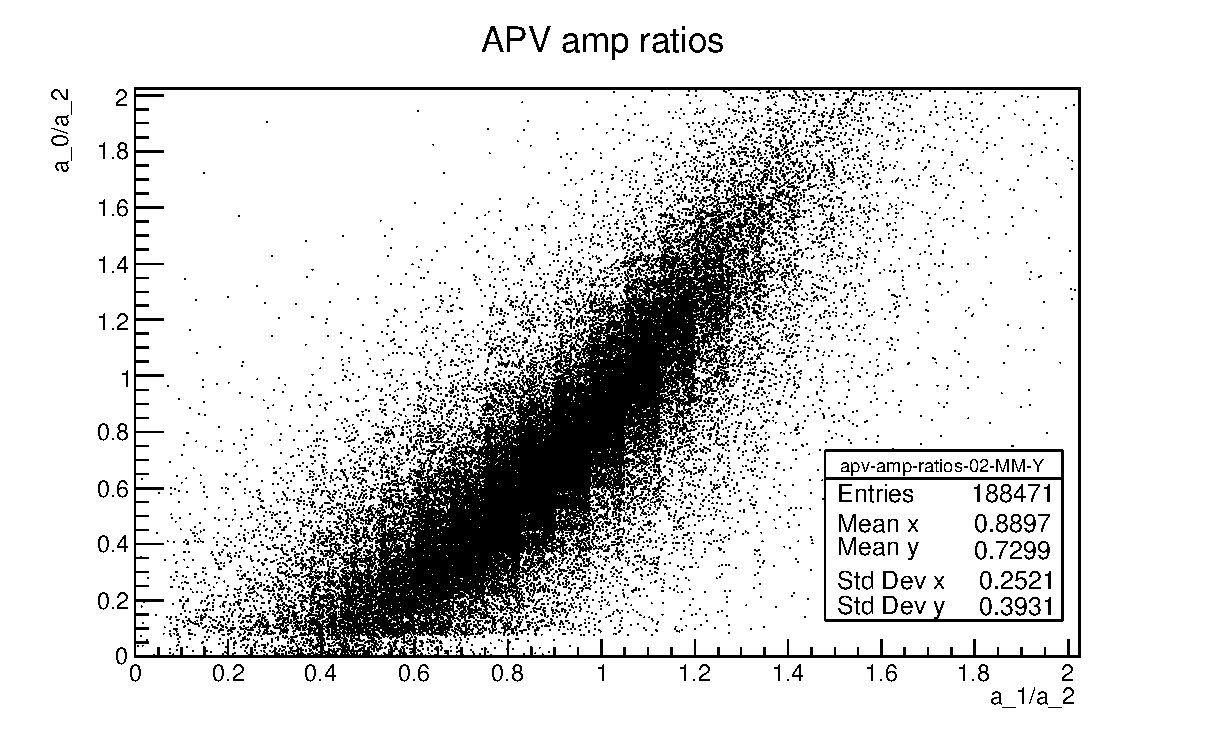
\includegraphics[width=0.45\linewidth]{images/illustrative/banana-example.eps}
    \caption{Пример распределения отношения амплитуд $r_{02}$ и $r_{12}$ переднего
    фронта сигнала микроструктурного детектора}
    \label{fig:banana-histogram}
\end{figure}

\subsection{Измерения от тонкостенных зарядовых трубок}

%Станции тонкостенных газоразрядных трубок предоставляют информацию
%о времени развития электронной лавины $t'$ в рабочем объёме конкретной
%трубки относительно времени срабатывания триггера. В $t'$ включено
%время пролёта частицы до трубки $\delta t$, которое для большинства
%релятивистских частиц (мюонов и электронов) принимается постоянным.
%Так, например, времяпролётная разница на дистанции в десять метров
%для электронов в $1~\text{ГэВ}$ и $100~\text{ГэВ}$ составляет
%менее $1~\text{пс}$, для мюонов -- менее $200~\text{пс}$, в то время
%как характерное время дрейфа лавины в трубке обычно составляет десятки
%наносекунд -- $20~\text{нс}$ для трубок диаметром $2~\text{мм}$
%и $50~\text{нс}$ для трубок $6~\text{мм}$. При принципиально-достижимом
%координатном разрешении в детекторах такого типа в $200~\text{мкм}$
%эта разница во временах для лептонов высоких энергий несущественна.
Станции тонкостенных газоразрядных трубок регистрируют время развития
электронной лавины $t'$ в рабочем объёме каждой трубки относительно
сигнала триггера. В это время включено также запаздывание
частицы $\delta t$, которое для большинства релятивистских частиц
практически постоянно. Так, например, различие
во времени пролёта на расстоянии десяти метров между электронами с
энергией $1~\text{ГэВ}$ и $100~\text{ГэВ}$ составляет менее $1~\text{пс}$,
а для мюонов~-- менее $200~\text{пс}$, тогда как характерное время
дрейфа лавины в трубке находится на уровне десятков наносекунд:
около $20~\text{нс}$ для трубок диаметром $2~\text{мм}$ и порядка
$50~\text{нс}$ для трубок диаметром $6~\text{мм}$. При достижимом
координатном разрешении таких детекторов на уровне менее $200~\text{мкм}$,
указанные различия во времени пролёта для лептонов высоких энергий
не имеют существенного значения.

%По этой причине $t'$ определяется главным образом временем $T$ дрейфа
%электронной лавины в разрядном промежутке трубки от ближайшей точки
%ионизации до катодной проволоки с расстоянием $R$, которое в свою очередь
%в наибольшей степени зависит от давления и плотности газовой смеси.
Таким образом, величина $t'$ определяется главным образом временем $T$
дрейфа электронов в разрядном промежутке трубки от ближайшей точки
ионизации до катодной проволоки.

%Таким образом зависимость $R(T)$, хотя и имеет нелинейный характер,
%хорошо поддаётся аппроксимации различными аналитическими моделями.
%Параметры такой модели и составляют необходимую калибровочную
%информацию применяемую при определении радиуса
%изохроной цилиндрической поверхности задаваемой временем срабатывания~$T$.
Функция $R(T)$ имеет нелинейный характер, однако хорошо аппроксимируется
различными аналитическими моделями. Параметры такой аппроксимации и
составляют необходимую калибровочную информацию, используемую при
определении радиуса изохронной цилиндрической поверхности, соответствующей
данному времени срабатывания~$T$.

На рисунке~\ref{fig:straws-rt} изображена гистограмма полученная для
трубки диаметром $6~\text{мм}$, находящейся
позади адронного калориметра с наложенными поверх гистограмм аппроксимациями
зависимости $R(T)$.
%\begin{figure}[ht]
%    \centering
%    \includegraphics[width=0.95\linewidth]{images/illustrative/ST-RT.jpg}
%    \caption{Распределение $R(T)$ для нескольких трубок станции ST
%    диаметром $6~\text{мм}$ (ось времени инверирована)}
%    \label{fig:straws-rt}
%\end{figure}
\begin{figure}
    \centering
    \includegraphics[width=0.33\linewidth]{images//illustrative/ST-RT-single-mono.png}
    \caption{Распределение $R(T)$ для нескольких трубок станции ST
    диаметром $6~\text{мм}$
    %, $R$ в мм, время в относительных единицах, ось времени инверирована
    }
    \label{fig:straws-rt}
\end{figure}
Большое количество срабатываний отстоящих от основной линии обусловлено
высоким фоном от вторичных частиц.

%Хотя определение радиуса изохронной поверхности таким образом представляет
%собой простую задачу (реализуемую при помощи единственного обработчика,
%применяющего калибровочные данные), последующее использование этой
%информации в
%алгоритмах трекинга требует привлечения нетривиальных
%алгоритмов либо на этапе предварительного поиска треков, либо
%в процессе подгонки параметров модели трека. В простейшем случае, проводят
%плоскость через оси трубок в одной координатной проекции, и отмечают
%линии пересечения изохронной поверхности с этой плоскостью. Получившиеся
%линии таким образом являются геометрическим местом возможного пересечения
%траектории частицы с плоскостью детектора с фиксированным разрешением.
%Поскольку для одной трубки таких линий образуется две, одной трубки
%недостаточно для определения координат частиц в одной проекции.
Хотя определение радиуса изохронной поверхности в таком подходе
представляет собой относительно простую задачу (реализуемую с помощью
единственного обработчика, использующего калибровочные данные),
дальнейшее применение этой информации в алгоритмах трекинга требует
привлечения более сложных методов -- как на этапе предварительного
поиска треков, так и при подгонке параметров модели трека. 

В простейшем случае через оси трубок в одной координатной проекции
проводится плоскость, и фиксируются линии пересечения изохронной
поверхности с этой плоскостью. Эти линии образуют геометрическое
место возможных точек пересечения траектории частицы с плоскостью
детектора при данном временном разрешении. Поскольку для одной трубки
возникают две такие линии, её информации недостаточно для определения
координаты частицы в одной проекции. Тем не менее, рассматривая показания
трековых детекторов в совокупности зачастую удаётся разрешить
возникающие неоднозначности. На рисунке~\ref{fig:evdisplay-new}
показана проекция пространственных примитивов изображающих
чувствительные объёмы детекторов MicroMega и станции трубок
совместно с допустимыми пределами разрешений (изображены
шириной $5\sigma$).

\begin{figure}[ht]
    \centerfloat{
        \includegraphics[width=0.5\linewidth]{images//illustrative/ST-evdisp-mono.png}
    }
    \caption{Реконструкция треков по показаниям MicroMega (повёрнуты на $45^{\circ}$)
    со станциями тонкостенных разрядных трубок с изображением
    координатных разрешений и гипотезы трека с ковариационными конусами}
    \label{fig:evdisplay-new}
\end{figure}

%\begin{figure}
%    \centering
%    \includegraphics[width=0.5\linewidth]{images/illustrative/ST-evdisp.jpg}
%    \caption{Реконструкция треков в SPA}
%    \label{fig:evdisplay-new}
%\end{figure}

Возможны и более сложные алгоритмы реконструкции, учитывающие
трёхмерную структуру изохронных поверхностей в рамках одной станции
тонкостенных трубок~\cite{straws-peshekhonov2015}.

\subsection{Алгоритмы аппроксимация треков}

Классическая задача восстановления трека по измеренным
координатам в NA64 решалась различными методами.
Наиболее актуальным является фильтр Калмана~\cite{kalman-1960},
реализованный библиотекой GenFit2~\cite{Genfit2_Rauch_2015}
в различных редакциях и с дополнениями оригинального алгоритма, из которых
наибольший практический интерес в контексте NA64
представляют
\acrshort{daf} (англ. \emph{deterministing annealing filter}~\cite{daf-track-fitting})
и \acrshort{krf}
(англ. \emph{Kalman filter with reference track}~\cite{krf-kalman-w-reference-track}).

Для подгонки параметров модели треков в условиях сложной геометрии
применяется \acrshort{krf}.
Его особенность по сравнению с оригинальным алгоритмом Калмана
состоит в том, что линеаризация функции описывающей движение
частицы выполняется не в малой окрестности координатного измерения, а
относительно заранее заданной опорной траектории,
обновляемой затем в несколько итераций. Этот приём позволяет снизить
систематические ошибки при аппроксимации трека в
неоднородном магнитном поле, с учётом эффектов множественного
рассеяния (например, при трассировке участка трека через калориметр).
Использование данного метода оправданно в сочетании с алгоритмами
поиска треков, которые задают разумное начальное приближение
для опорной траектории. % -- таких, как CATS~\cite{catsc-nim}.

\acrshort{daf} решает иную задачу: выбор согласованного подмножества
измерений в условиях неоднозначностей и шумов. В
его основу положено назначение весов отдельным координатным измерениям
с последующим итеративным обновлением. Таким образом, вначале все
измерения вносят вклад в гипотезу о треке частицы, затем, в течение
нескольких итераций, веса
асимптотически сходятся к самосогласованной гипотезе.
В пределе это приводит к отбору хитов, принадлежащих
правдоподобной гипотезе с эффективным исключением ложных
срабатываний.

\subsection{Задача предварительного поиска треков}

%Задача предварительного поиска треков (англ. \emph{pattern recognition})
%состоит в выборе таких комбинаций пространственных объектов соответствующих
%отдельным измерениям, которые с заданной
%степенью правдоподобия могут образовывать трек частицы.
Задача предварительного поиска треков % (англ. \emph{pattern recognition})
заключается в отборе таких комбинаций пространственных объектов,
соответствующих отдельным измерениям детектора, которые с заданной
степенью правдоподобия могут образовывать трек частицы.


%Среди множества существующих на сегодняшний день алгоритмов предварительного
%поиска треков~\cite{MankelTracking}, интерес представляет алгоритм
%CATS~\cite{catsc-JINR, catsc-discrete, catsc-nim, catsc-disto},
%(англ. \emph{cellular automata track search} -- в разное время авторы
%публиковали его формализацию в терминах <<эластичных>> нейронных сетей,
%и клеточных автоматов), который допускает весьма общую
%формулировку в силу независимости по отношению к конкретным
%геометрическим свойствам входных данных.
Среди многочисленных алгоритмов предварительного поиска~\cite{MankelTracking}
интерес представляет метод CATS\footnote{В различных публикациях
он излагался как в терминах <<эластичных>> нейронных сетей,
так и в формализме клеточных автоматов.}
(англ. \emph{cellular automata track search})~\cite{catsc-JINR, catsc-discrete, catsc-nim, catsc-disto}.
Алгоритм допускает весьма общую формулировку в силу независимости по
отношению к конкретным геометрическим свойствам входных данных.

Формально задача, решаемая алгоритмом, может быть представлена следующим образом.
Пусть имеется
набор объектов $h_1,h_2, ...h_n$ (англ. \emph{hit}). Требуется найти такие
последовательности $(h_i,h_j,...h_m)$, для которых любая тройка
элементов $(h_{i-1},h_{i},h_{i+1})$ удовлетворяет заданному
условию $F(h_{i-1},h_{i},h_{i+1})=1$.
Основная идея состоит в эффективной стратегии обхода
объектов~$h$, позволяющей в большинстве случаев избежать прямого перебора
всех возможных комбинаций. Для этого алгоритм опирается на
топологическую информацию о <<слоях>> связанных с каждым
объектом~$h$. Каждому объекту сопоставляется
внутреннее состояние, обновляемых за конечно число итераций согласно
определённому правилу.

Пример работы алгоритма показан на рисунке~\ref{fig:catsc-nim},
где приведены начальное и конечное состояния графа для
синтетических данных.

\begin{figure}
    \centerfloat{
        \hfill
        \subcaptionbox{Начальное состояние}{
            \includegraphics[width=0.45\linewidth]{images//illustrative/catsc-quote-it1.png}}
        \hfill
        \subcaptionbox{Конечное состояние}{
            \includegraphics[width=0.45\linewidth]{images//illustrative/catsc-quote-it6.png}
        }
        \hfill
    }
    \legend{Слои отмечены пунктирными
    линиями, объекты $h$ изображены кругами, рёбра между парами
    объектов~--- сплошными линиями, а увеличенная толщина линии указывает
    на больший вес соответствующей пары.}
    \caption{Пример работы клеточного автомата CATS~\cite{catsc-nim}}
    \label{fig:catsc-nim}
\end{figure}

В простейшем случае, в качестве объектов $h$ выбираются пространственные
точки, а условием $F$ является условие на максимальный пространственный
между ними $F(h_{i-1},h_{i},h_{i+1}): \angle(h_{i-1}h_i) (h_i h_{i+1}) < \theta_{th}$.

В результате время работы алгоритма оказывается существенно ниже
прямого перебора, в худшем случае ($\theta_{th} =\pi$) имея
сложность $\mathcal{O}(Ln^3)$, где $L$ -- число слоёв,
и $n$ -- число объектов $h$. Практически, сложность регулируется
функцией-фильтром, и при трудоёмкости фильтра~$\mathcal{O}(1)$ алгоритм
имеет сложность $\mathcal{O}(Ln^2)$. Наивный перебор троек $h$
с фильтрующей функцией дающей в среднем $d$ объектов в следующем слое
имеет сложность $\mathcal{O}(n^3 d^{L-3})$. Без фильтрующей функции
максимальная сложность возрастает экспоненциально $\mathcal{O}(n^L)$,
однако главное преимущество CATS перед наивной реализацией состоит
в устранении экспоненциального роста памяти, необходимой для хранения
гипотез. Алгоритм сводит задачу к итеративному однонаправленному обходу
двунаправленного графа без рекурсии.

В оригинальных работах~\cite{catsc-JINR, catsc-discrete, catsc-nim, catsc-disto}
$h_i$ рассматриваются как пространственные точки $h_i:=\vec{r}_i$, или кортежи из
координат и времени $h_i:=(\vec{r}_i,t_i)$, в то время как алгоритм сам по себе
не подразумевает какого-то конкретного набора свойств, а требует
только того, чтобы определена функция $F:h_{1,2,3} \rightarrow \{0,1\}$.

Дополнением оригинального алгоритма является определение весовых
коэффициентов возвращаемых функцией-фильтром, то есть в более общем
случае $F: F(h_{1,2,3}) =w_j, ~w_j \in \mathbb{R_1}$. Кроме того, после
конструирования графа связности, стратегия извлечения гипотез (обхода точек)
может допускать различные формы, что в оригинальных работах не
рассматривается. В частности, в случае когда одна и более гипотез $T_p, T_q$
претендуют на один и тот же сегмент $T_p \cap T_q = (h_i, h_j)$ выбор в пользу
той или иной гипотезы целесообразно бывает разрешать руководствуясь различными
критериями. Стратегии обхода результирующего графа реализованы в виде
программных модулей.

\subsection{Результаты}

Детекторы и система сбора данных NA64 принципиально способны
регистрировать события с высокой множественностью треков
(до нескольких сотен). Однако, без применения алгоритмов
предварительного выбора гипотез, восстановление
трека алгоритмами типа \acrshort{daf} позволяет получить усреднённое представление
о треках частиц, с потерей существенной части физической информации.
На рисунке~\ref{fig:muon-momenta-test-histogram}
приведён спектр треков мюонов, восстановленных с помощью алгоритма
\acrshort{daf} при высокой интенсивности пучка
(порядка $10^6$ мюонов в секунду).
\begin{figure}[h]
    \centerfloat{
        \includegraphics[width=0.65\linewidth]{images//illustrative/momentum-reco-example.png}
    }
    \caption{Спектр мюонов реконструированных алгоритмом \acrshort{daf} без
    предварительного выбора гипотез}
    \label{fig:muon-momenta-test-histogram}
\end{figure}
Пьедестал спектра в основном соответствует случайной сходимости
алгоритма на правдоподобных комбинациях координатных измерений,
без учёта конкурирующих гипотез и дополнительных предположений о
правдоподобии.

Использование алгоритма CATS для выделения треков частиц
позволяет эффективно исключить некорректные гипотезы, согласно
некоторому геометрическому критерию. При заданной принадлежности
объектов $h_p,h_q,h_r$ идущим по порядку
слоям $h_p\in l_{i-1}, h_i \in l_i, h_p\in l_{i+1}$ критерий $F(h_{p}, h_q, h_{r}) \in [0,1]$ может включать произвольное условие.

\subsection{Результаты CATS(C) на модели данных Belle~II}

В качестве примера, помимо простейшего теста на принадлежность угла
$\angle(h_p,h_q),(h_q,h_r)$ заданному диапазону, можно рассмотреть
постановку задачи в соленаодиальном поле баррельной части коллайдерного
детектора, в рамках которой функция-фильтр $F$ должна проверять
гипотезу о спиральной траектории заряженных частиц в смысле некоторых
регулярных геометрических свойств. Например, в цилиндрической системе
координат $(\rho, \phi, z)$, выбирая попарные комбинации из триплета $h_{p}, h_q, h_{r}$,
можно проверять шаг $\lambda_{ij} = \Delta z_{ij}/\Delta \phi_{ij}$
на приблизительное равенство относительно некоторого порога $\epsilon$:
\begin{align}
    F(h_{p}, h_q, h_{r}) = |\lambda_{12} / \lambda_{23} - 1| <\epsilon ~
    \wedge |\lambda_{12} / \lambda_{13} - 1| <\epsilon.
\end{align}

Результаты моделирования в геометрии Belle~II~\cite{belle-ii} изображены на
рисунке~\ref{fig:belle-ii-mc-event}.
\begin{figure}[ht]
    \centerfloat{
        \includegraphics[width=1\linewidth]{images//illustrative/belle-ii-mc-event.png}
    }
    \legend{Поверх схематичного изображения детекторов
внутреннего и внешнего трекера зелёным нанесены точки, соответствующие
измерениям детекторов $h$, синими линиями соединены найденные треки,
соответствующие истинным траекториям, реконструированным алгоритмом;
серым -- комбинации отвечающие ложным гипотезам.}
    \caption{Результат применения реализации CATS(C) на данных \acrshort{mc}-моделирования
    одного сособытия геометрии детектора Belle II~\cite{belle-ii} 
    (автор -- С.~Герасимов}
    \label{fig:belle-ii-mc-event}
\end{figure}

На рисунке \ref{fig:belle-ii-catsc} приведены результаты моделирования
для Belle~II, откуда для заданного уровня статистической значимости можно получить
ограничения на значения различных порогов функции-фильтра.
Заметно, что значения, соответствующие истинным трекам размываются благодаря множественному рассеянию.

\begin{figure}
    \centerfloat{
        \subcaptionbox{Отношение спирального шага $\lambda_{12}/\lambda_{23}$}{\includegraphics[width=0.32\linewidth]{images//illustrative/pitch-ratios.png}}
        \subcaptionbox{Продольный угол $\alpha_{12-23}$}{\includegraphics[width=0.3\linewidth]{images//illustrative/belle-ii-catsc-opening-angle.png}}
        \subcaptionbox{Разница спиральных шагов
    $\lambda_{12} - \lambda_{23}$}{\includegraphics[width=0.32\linewidth]{images//illustrative/belle-ii-catsc-pitch-delta.png}}
    }
    \legend{Зелёным цветом выделены значения,
    соответствующие истинным трекам, комбинаторный фон обозначен жёлтым}
    \caption{Распределения спиральных геометрических характеристик триплетов,
    по результатам \acrshort{mc}-моделирования
    Belle~II для оценки мощности критерия~(С.~Герасимов)}
    \label{fig:belle-ii-catsc}
\end{figure}

\subsection{Результаты CATS(C) данных $\text{NA64}\mu$}

Результаты применения алгоритма для реконструкции треков $\text{NA64}\mu$ приведены на
рисунке~\ref{fig:cats-impact-na64}.
\begin{figure}[ht]
    \centerfloat{
        \hfill
        \subcaptionbox{}{
            \includegraphics[width=0.49\linewidth]{images//illustrative/catsc-impact.png}
        }
        \hfill
        \subcaptionbox{}{
                \includegraphics[width=0.49\linewidth]{images//illustrative/catsc-impact-2.png}
        }
        \hfill
    }
    \caption{Распределение импульсов частиц NA64mu реконструированных при
    помощи DAF без применения CATS(C) и при помощи KRF после CATS(C)
    до (MS1) и после (MS2) основного магнита спектрометра NA64mu~(автор -- M.~Tuzi)}
    \label{fig:cats-impact-na64}
\end{figure}
В постановке NA64mu применение алгоритма для предварительного отбора гипотез треков
особенно важно, поскольку участок установки MS2 находится после электромагнитного
калориметра, и трекер должен разрешать траектории при повышенной
загрузке (в среднем $\simeq 10$ треков на событие против $\simeq 1.4$ в MS1)
от вторичных частиц после ECAL.

При консервативной оценке пороги для углов или спирального шага
регулируют в основном количество избыточных гипотез найденных алгоритмом, которые
затем отсеивают при подгонке треков и проверки более строгих гипотез. Избыточные
гипотезы можно ограничить на основе оценок порогов полученных с
применением \acrshort{mc}-моделирования, или при помощи консервативных
геометрических оценок.

В некоторых случая можно прибегнуть к упрощённому рассмотрению.
Рисунок~\ref{fig:na64-cutoff-angle} иллюстрирует распределение углов
для допустимых триплетов $h$ в пределах $3\sigma$, где $\sigma$ -- пространственное
разрешение одной станции. Видна существенная (вплоть до кратности $\times5$) разница
углового порога.
\begin{figure}[ht]
    \centering
    \includegraphics[width=0.5\linewidth]{images//illustrative/na64-cutoff-effic.png}
    \caption{Распределение углов для всех возможных комбинаций при учёте разрешения
    отдельных станций трекера MS2 NA64mu~(M.Tuzi)}
    \label{fig:na64-cutoff-angle}
\end{figure}

\subsection{Количественные оценки качества восстановления треков}

%Задача восстановления треков частиц по данным зачастую формулируется
%как минимизация функционала, в котором в качестве метрического значения
%выбирается величина, пропорциональная отклонению ожидаемых значений
%от фактически измеренных. Для многих детекторов статистика таких
%отклонений (ошибок), отнесённых к абсолютному разрешению детектора,
%подчиняется распределению~$\chi^2$.

%\begin{figure}[ht]
%    \centering
%    \includegraphics[width=1\linewidth]{images//illustrative/na64-p-value-before-truly.png}
%    \includegraphics[width=1\linewidth]{images//illustrative/na64-pvalue-before.png}
%    \caption{Распределение $p_{\chi^2}$ реконструированных треков для плечей мюонного спектрометра NA64 до и после учёта wire layout~(M.Tuzi)}
%    \label{fig:na64-muon-p-value-distribution}
%\end{figure}

Важным фактором, влияющим на качество восстановления треков, является
соответствие предполагаемых положений детекторов фактическим. Для
оценки этого соответствия в случае индивидуальных детекторов строят
распределения координатных невязок (англ. \emph{residuals}) в
системе локальных координат, связанной с детектором.
Для стриповых и проволочных детекторов (измеряющих координату в
одном направлении) используют одно направление ($u$), выбираемое
соответствующим измеряемой координате, второе обычно
перпендикулярно ему.

При ориентации плоскости перпендикулярно пучку распределение невязок
характеризует ошибку в определении позиции центра
координатной плоскости детектора в поперечных координатах (вдоль $u$).
Для получения более детализированной картины строят
распределение $\delta u/dv$, естественно характеризующее ошибку в определении
угла поворота, перпендикулярного направлению пучка. Распределение
$\delta u/du$ характеризует ошибку в определении продольной координаты.

На рисунке~\ref{fig:residuals-example} показан пример комплексного
графика, характеризующего распределение невязок $\delta u$ против $v$.
\begin{figure}[ht]
    \centering
    \includegraphics[width=0.95\linewidth]{images/illustrative/alignment-example.png}
    \caption{Комплексный график иллюстрирующий распределение координатных
    невязок $\delta u /v$ для плоскости X первой станци MicroMega}
    \label{fig:residuals-example}
\end{figure}

Такое изображение координатных невязок можно использовать, в частности,
в процедуре выравнивания детекторов по \emph{несмещённым} невязкам, когда
среди всего набора выбирается пара опорных детекторов $P_1,~P_2$, по отношению
к которым производят итеративное выравнивание. Включая в процедуру
реконструкции по одному детектору последовательно, для каждого уточняют
значения позиций и углов на основе распределений подобных изображённым
на рисунке~\ref{fig:residuals-example} при условии, что рассматриваемый
в данный момент детектор не используется для реконструкции треков (однако,
программный комплекс рассчитывает для него координатные невязки).

Подобные изображения координатных невязок используются, в частности,
в процедуре выравнивания детекторов по \emph{несмещённым} невязкам.
В такой процедуре из всего набора выбирается пара опорных детекторов,
относительно которых проводится итеративное выравнивание.
Для каждого отдельного детектора уточняют положения и углы на основе распределений,
подобных показанным на рисунке~\ref{fig:residuals-example}, при условии,
что данный детектор не используется для реконструкции треков (однако
программный комплекс вычисляет для него координатные невязки). После
выравнивания очередного детектора, он добавляется к опорным, и переходят
к следующему.

Процедура выравнивания по \emph{смещённым} невязкам, напротив,
предполагает включение всех корректируемых детекторов в реконструкцию трека.
В этом случае линеаризованные невязки образуют блочную матрицу,
которую можно использовать для решения \acrshort{sle}.

В программном окружении реализованы инструменты
для обеих процедур физического выравнивания и оценивания качества
реконструкции треков частиц. Инструменты для выравнивания по
несмещённым невязкам (графики и регрессионные модели) реализованы
в парадигме отдельных обработчиков ковейерного паттерна, выравнивание
по смещённым невязкам реализовано в виде специализированных
обработчиков и специализированной утилиты для помещения их вывода
на вход процедуры обращения блочных матрицы
Millipede~II~\cite{millipede-blobel2009}.

На рисунке~\ref{fig:na64-muon-p-value-distribution} показаны распределения $p$-значений
(интегральных вероятностей $\chi^2$) в плече MS1. Вид этого распределения
используется для косвенной оценки качества работы трекера. В случае полного
соответствия фактических разрешений детекторов установки номинальным,
распределение должно быть плоским. Увеличение популяции справа
($p_{\chi^2} \rightarrow 1{,}0$) означает, что разрешение одной или нескольких
станций оценивается пессимистически (фактическое меньше ожидаемого).
\begin{figure}[ht]
    \centering
    \includegraphics[width=0.5\linewidth]{images/na64-ms1-p-value-before.png}
%    \includegraphics[width=0.5\linewidth]{na64-muon-p-value-ms1-dist-after.png}
    \caption{Распределение $p_{\chi^2}$ реконструированных треков в плече MS1 мюонного спектрометра NA64 после выравнивания~(M.Tuzi)}
    \label{fig:na64-muon-p-value-distribution}
\end{figure}

Наблюдаемое на рисунке слева увеличение наблюдений свидетельствует
о наличии факторов, неучтённых моделью трека: неудовлетворительного
геометрического выравнивания, снижения эффективности за счёт
дефектов детектора, большего вклада множественного
рассеяния и т.~д.
На приведённой гистограмме около 7\% треков отклоняются как не
соответствующие уровню значимости $\alpha = 0{,}01$.
